%%%%%%%%%%%%%%%%%%%%%%%%%%%%%%%%%%%%%%%%%%%%%%%%%%%%%%%%%%%%
%%  Class 1, NE 155
%%

\documentclass[xcolor=x11names,compress]{beamer}

\definecolor{CoolBlack}{rgb}{0.0, 0.18, 0.39}
%% General document %%%%%%%%%%%%%%%%%%%%%%%%%%%%%%%%%%
\usepackage{graphicx}
\usepackage{tikz}
\usetikzlibrary{decorations.fractals}
\usepackage{hyperref}
%%%%%%%%%%%%%%%%%%%%%%%%%%%%%%%%%%%%%%%%%%%%%%%%%%%%%%

%% Beamer Layout %%%%%%%%%%%%%%%%%%%%%%%%%%%%%%%%%%
\useoutertheme[subsection=false,shadow]{miniframes}
\useinnertheme{default}
\usefonttheme{serif}
\usepackage{palatino}
\usepackage{tabu}
% Links
\usepackage{hyperref}
\definecolor{links}{HTML}{003262}
\hypersetup{colorlinks,linkcolor=,urlcolor=links}

% addition of color
\usepackage{xcolor}
\definecolor{CoolBlack}{rgb}{0.0, 0.18, 0.39}
\definecolor{byellow}{rgb}{0.55037, 0.38821, 0.06142}
\definecolor{dgreen}{rgb}{0.,0.6,0.}
\definecolor{RawSienna}{cmyk}{0,0.72,1,0.45}
\definecolor{forestgreen(web)}{rgb}{0.13, 0.55, 0.13}
\definecolor{cardinal}{rgb}{0.77, 0.12, 0.23}

\setbeamerfont{title like}{shape=\scshape}
\setbeamerfont{frametitle}{shape=\scshape}

\setbeamercolor*{lower separation line head}{bg=CoolBlack}
\setbeamercolor*{normal text}{fg=black,bg=white}
\setbeamercolor*{alerted text}{fg=dgreen} % just testing; I think this looks better
\setbeamercolor*{example text}{fg=black}
\setbeamercolor*{structure}{fg=black}

\setbeamercolor*{palette tertiary}{fg=black,bg=black!10}
\setbeamercolor*{palette quaternary}{fg=black,bg=black!10}

% Margins
\usepackage{changepage}

\mode<presentation>
{
  \definecolor{berkeleyblue}{HTML}{003262}
  \definecolor{berkeleygold}{HTML}{FDB515}
  \usetheme{Boadilla}      % or try Darmstadt, Madrid, Warsaw, Boadilla...
  %\usecolortheme{dove} % or try albatross, beaver, crane, ...
  \setbeamercolor{structure}{fg=berkeleyblue,bg=berkeleygold}
  \setbeamercolor{palette primary}{bg=berkeleyblue,fg=white} % changed this
  \setbeamercolor{palette secondary}{fg=berkeleyblue,bg=berkeleygold} % changed this
  \setbeamercolor{palette tertiary}{bg=berkeleyblue,fg=white} % changed this
  \usefonttheme{structurebold}  % or try serif, structurebold, ...
  \useinnertheme{circles}
  \setbeamertemplate{navigation symbols}{}
  \setbeamertemplate{caption}[numbered]
  \usebackgroundtemplate{}
}
%---

\renewcommand{\(}{\begin{columns}}
\renewcommand{\)}{\end{columns}}
\newcommand{\<}[1]{\begin{column}{#1}}
\renewcommand{\>}{\end{column}}

% adding slide numbers
\addtobeamertemplate{navigation symbols}{}{%
    \usebeamerfont{footline}%
    \usebeamercolor[fg]{footline}%
    \hspace{1em}%
    \insertframenumber/\inserttotalframenumber
}

% equation stuff
\newcommand{\Macro}{\ensuremath{\Sigma}}
\newcommand{\Sn}{\ensuremath{S_N} }
\newcommand{\vOmega}{\ensuremath{\hat{\Omega}}}
\usepackage{mathrsfs}
\usepackage[mathcal]{euscript}
\usepackage{amssymb}
\usepackage{amsthm}
\usepackage{epsfig}
\usepackage{amsmath}
%%%%%%%%%%%%%%%%%%%%%%%%%%%%%%%%%%%%%%%%%%%%%%%%%%
% title stuff for footer
\title{NE 155}
\author{R.\ N.\ Slaybaugh}
\date{January 23, 2014}

\begin{document}

%%%%%%%%%%%%%%%%%%%%%%%%%%%%%%%%%%%%%%%%%%%%%%%%%%%%%%
%%%%%%%%%%%%%%%%%%%%%%%%%%%%%%%%%%%%%%%%%%%%%%%%%%%%%%
\begin{frame}
\title{NE 155\\Introduction to Numerical Simulations in Radiation Transport}
\subtitle{Lecture 2: Computing}
\titlepage
\end{frame}

%%%%%%%%%%%%%%%%%%%%%%%%%%%%%%%%%%%%%%%%%%%%%%%%%%%%%%
%%%%%%%%%%%%%%%%%%%%%%%%%%%%%%%%%%%%%%%%%%%%%%%%%%%%%%
\begin{frame}{Outline}
%\tableofcontents
\begin{enumerate}
\item History and terminology
%  - define flops as measure of what we care about
%  - chronological highlights of a few machines; show pictures, state details
\item Basic computer architecture
%  - hardware v software; we're talking about hardware now but the rest of the class will focus on software. We will care a little bit about the interface
%  - definitions
%  - Moore's law
\item Introduction to Parallelism
%  - basic considerations
%  - types of parallelism
%  - speedup
%  - increase in use and potential
%  - current status
\item Current supercomputers
%  - Moore's law continuation?
%  - GPUs
%  - mic chips
%  - What happens may have a large impact on algorithms
\end{enumerate}
\end{frame}

%%%%%%%%%%%%%%%%%%%%%%%%%%%%%%%%%%%%%%%%%%%%%%%%%%%%%%
%%%%%%%%%%%%%%%%%%%%%%%%%%%%%%%%%%%%%%%%%%%%%%%%%%%%%%
\begin{frame}{How do we measure utility?\footnote{en.wikipedia.org}}

\textbf{IPS} (Instructions Per Second) is a measure of a computer's processor speed. IPS can be useful when comparing performance between processors made from a similar architecture, but are difficult to compare between CPU architectures

\vspace*{1 em}
\textbf{Clock rate} typically refers to the frequency at which a CPU is running. It is measured in the SI unit Hertz.

\vspace*{1 em}
\textbf{FLOPS} (FLoating-point Operations Per Second) is a measure of computer performance, useful in fields of scientific calculations that make heavy use of floating-point calculations. 
\end{frame}

%%%%%%%%%%%%%%%%%%%%%%%%%%%%%%%%%%%%%%%%%%%%%%%%%%%%%%
%%%%%%%%%%%%%%%%%%%%%%%%%%%%%%%%%%%%%%%%%%%%%%%%%%%%%%
\section{\scshape History}
\subsection{History}
\begin{frame}{Computing Machines, Origins}
\begin{figure}
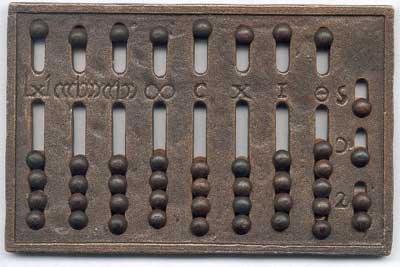
\includegraphics[height=2.25in,clip]{RomanAbacus}
\caption{Roman Abacus, http://history-computer.com/CalculatingTools/abacus.html}
\end{figure}

\end{frame}

%%%%%%%%%%%%%%%%%%%%%%%%%%%%%%%%%%%%%%%%%%%%%%%%%%%%%%
%%%%%%%%%%%%%%%%%%%%%%%%%%%%%%%%%%%%%%%%%%%%%%%%%%%%%%
\begin{frame}{Early Development of Computing}

\begin{figure}
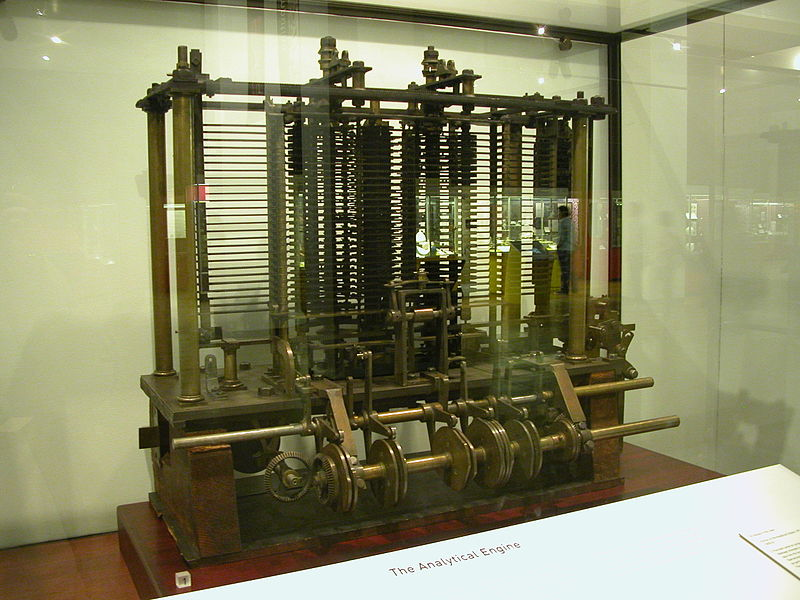
\includegraphics[height=2in,clip]{BabbageDiffMachine}
\caption{Reconstruction of Babbage's Analytical Engine, the first general-purpose programmable computer, http://en.wikipedia.org/wiki/History\_of\_computing\_hardware
\#Punched\_card\_data\_processing}
\end{figure}

\end{frame}

%%%%%%%%%%%%%%%%%%%%%%%%%%%%%%%%%%%%%%%%%%%%%%%%%%%%%%
%%%%%%%%%%%%%%%%%%%%%%%%%%%%%%%%%%%%%%%%%%%%%%%%%%%%%%
\begin{frame}{First Electromechanical Computers}

\begin{figure}
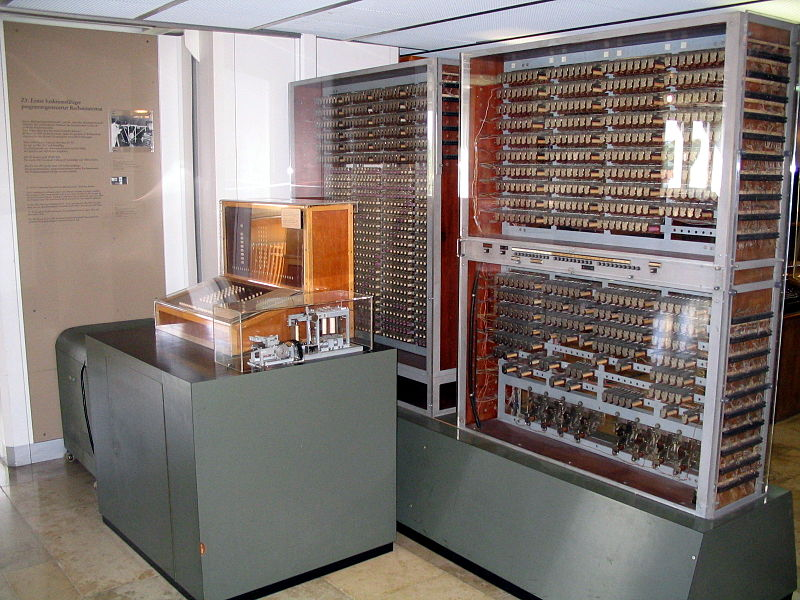
\includegraphics[height=2in,clip]{Z3DeutschesMuseum}
\caption{Zuse Z3 replica on display at Deutsches Museum in Munich, en.wikipedia.org/wiki/Z3\_(computer)}
\end{figure}

\end{frame}

%%%%%%%%%%%%%%%%%%%%%%%%%%%%%%%%%%%%%%%%%%%%%%%%%%%%%%
%%%%%%%%%%%%%%%%%%%%%%%%%%%%%%%%%%%%%%%%%%%%%%%%%%%%%%
\begin{frame}{Stored Programs}

\begin{figure}
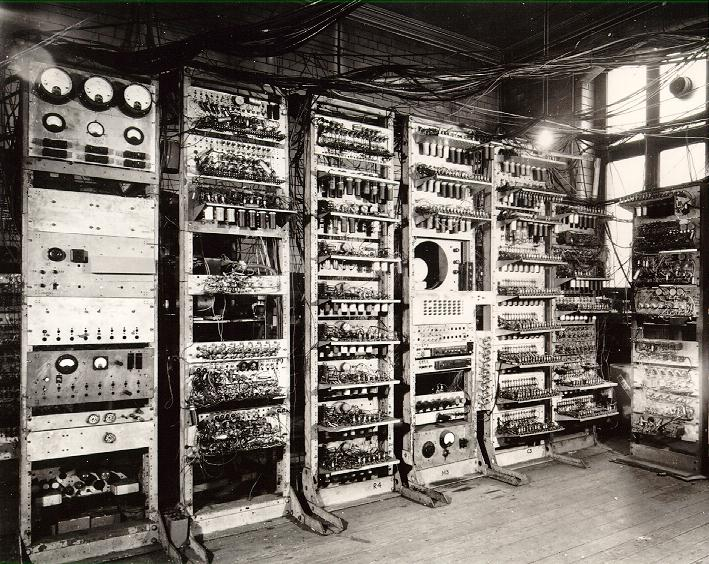
\includegraphics[height=2in,clip]{ManchesterMark1}
\caption{The Manchester Mark 1 was one of the world's first stored-program computers, http://www.computer50.org/mark1/ip-mm1.mark1.html}
\end{figure}

\end{frame}

%%%%%%%%%%%%%%%%%%%%%%%%%%%%%%%%%%%%%%%%%%%%%%%%%%%%%%
%%%%%%%%%%%%%%%%%%%%%%%%%%%%%%%%%%%%%%%%%%%%%%%%%%%%%%
\begin{frame}{Microprogramming, Magnetic Storage, Transistors}
\begin{itemize}
\item 1951: realization that CPUs can be controlled by a miniature, highly specialized computer program in high-speed ROM
\item 1954: magnetic core memory was rapidly displacing most other forms of temporary storage
\item 1956: IBM introduced the first disk storage unit: using 50 24-inch metal disks, it stored 5 MB of data for \$10,000 per MB (\$90,000 in 2014 \$s)
\item 1947: invention of the bipolar transistor; this replaced vacuum tubes by 1955 $\rightarrow$ ``Second Generation" of computer designs
\end{itemize}
\end{frame}

%%%%%%%%%%%%%%%%%%%%%%%%%%%%%%%%%%%%%%%%%%%%%%%%%%%%%%
%%%%%%%%%%%%%%%%%%%%%%%%%%%%%%%%%%%%%%%%%%%%%%%%%%%%%%
\begin{frame}{Supercomputers}

\begin{figure}
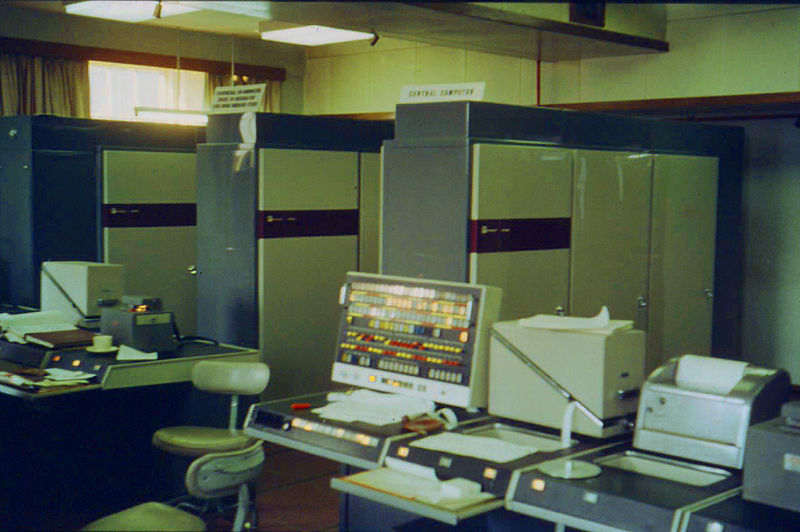
\includegraphics[height=2in,clip]{Atlas1963}
\caption{The University of Manchester Atlas 1963, http://en.wikipedia.org/wiki/History\_of\_computing\_hardware
\#Punched\_card\_data\_processing}
\end{figure}

\end{frame}

%%%%%%%%%%%%%%%%%%%%%%%%%%%%%%%%%%%%%%%%%%%%%%%%%%%%%%
%%%%%%%%%%%%%%%%%%%%%%%%%%%%%%%%%%%%%%%%%%%%%%%%%%%%%%
\begin{frame}{Integrated Circuit}
With the advent of the \alert{transistor} and the work on semi-conductors generally, it now seems possible to envisage electronic equipment in a solid block with no connecting wires. The block may consist of layers of insulating, conducting, rectifying and amplifying materials, the \alert{electronic functions being connected directly} by cutting out areas of the various layers.\\
\vspace*{1.5 em}
\hspace*{0.5 in}Geoffrey W.A. Dummer, Royal Radar Establishment of the Ministry of Defence, 1952

\end{frame}

%%%%%%%%%%%%%%%%%%%%%%%%%%%%%%%%%%%%%%%%%%%%%%%%%%%%%%
%%%%%%%%%%%%%%%%%%%%%%%%%%%%%%%%%%%%%%%%%%%%%%%%%%%%%%
\begin{frame}{Generations 4-6}
\begin{itemize}
\item Very large scale integration of devices on chip
\item C and FORTRAN programming languages
\item UNIX operating system (Bell labs, Berkeley)
\item Large scale parallel processing; supercomputing centers
\item Shared and distributed memory
\item Parallel/vector shared/distributed memory combinations
\item High speed networking
\end{itemize}
\end{frame}

%%%%%%%%%%%%%%%%%%%%%%%%%%%%%%%%%%%%%%%%%%%%%%%%%%%%%%
%%%%%%%%%%%%%%%%%%%%%%%%%%%%%%%%%%%%%%%%%%%%%%%%%%%%%%
\section{\scshape Computer Architecture}
\subsection{Computer Architecture}
\begin{frame}{Computer Architecture}
 \begin{figure}
   \begin{center}
     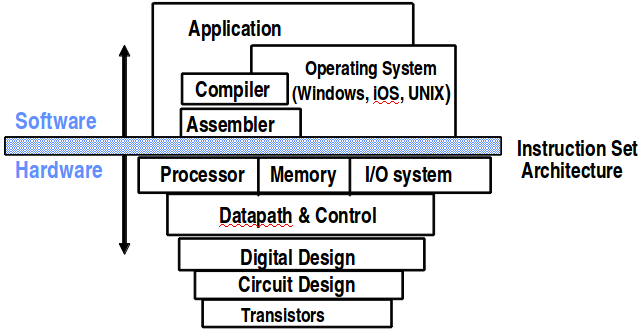
\includegraphics[height=2.25in,clip]{ComputerArchitecture}
   \end{center}
 \end{figure}
\end{frame}

%%%%%%%%%%%%%%%%%%%%%%%%%%%%%%%%%%%%%%%%%%%%%%%%%%%%%%
%%%%%%%%%%%%%%%%%%%%%%%%%%%%%%%%%%%%%%%%%%%%%%%%%%%%%%
\begin{frame}{Components}
 \begin{figure}
   \begin{center}
     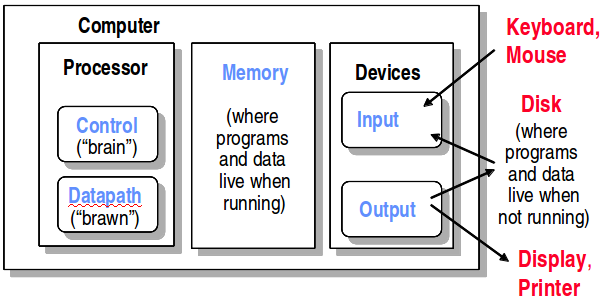
\includegraphics[height=2.25in,clip]{Components}
   \end{center}
 \end{figure}
\end{frame}

%%%%%%%%%%%%%%%%%%%%%%%%%%%%%%%%%%%%%%%%%%%%%%%%%%%%%%
%%%%%%%%%%%%%%%%%%%%%%%%%%%%%%%%%%%%%%%%%%%%%%%%%%%%%%
%\begin{frame}{Types of Memory}
%\begin{itemize}
%\item \textbf{Read-only memory} (ROM): storage medium in which data cannot be modified, so it is mainly used to distribute firmware 
%\item \textbf{Random Access Memory} (RAM): allows stored data to be accessed directly in any random order\footnote{Many computer systems have a memory hierarchy consisting different systems referred to collectively as ``RAM". The various subsystems can have very different access times.}
%\item Other data storage media only read and write data consecutively (time impact)
%\end{itemize}
%\end{frame}

%%%%%%%%%%%%%%%%%%%%%%%%%%%%%%%%%%%%%%%%%%%%%%%%%%%%%%
%%%%%%%%%%%%%%%%%%%%%%%%%%%%%%%%%%%%%%%%%%%%%%%%%%%%%%
\begin{frame}{Moore's ``Law"}
The number of transistors on integrated circuits doubles approximately every 18 months. 

\begin{columns}
  \begin{column}{0.7\textwidth}
\begin{itemize}
\item In 1965 Gordon E. Moore described this trend and predicted it to hold for at least 10 years
\item He worked at Intel
\item The trend has held, but is expected to change around now...
\end{itemize}
  \end{column}
  \begin{column}{0.3\textwidth}
    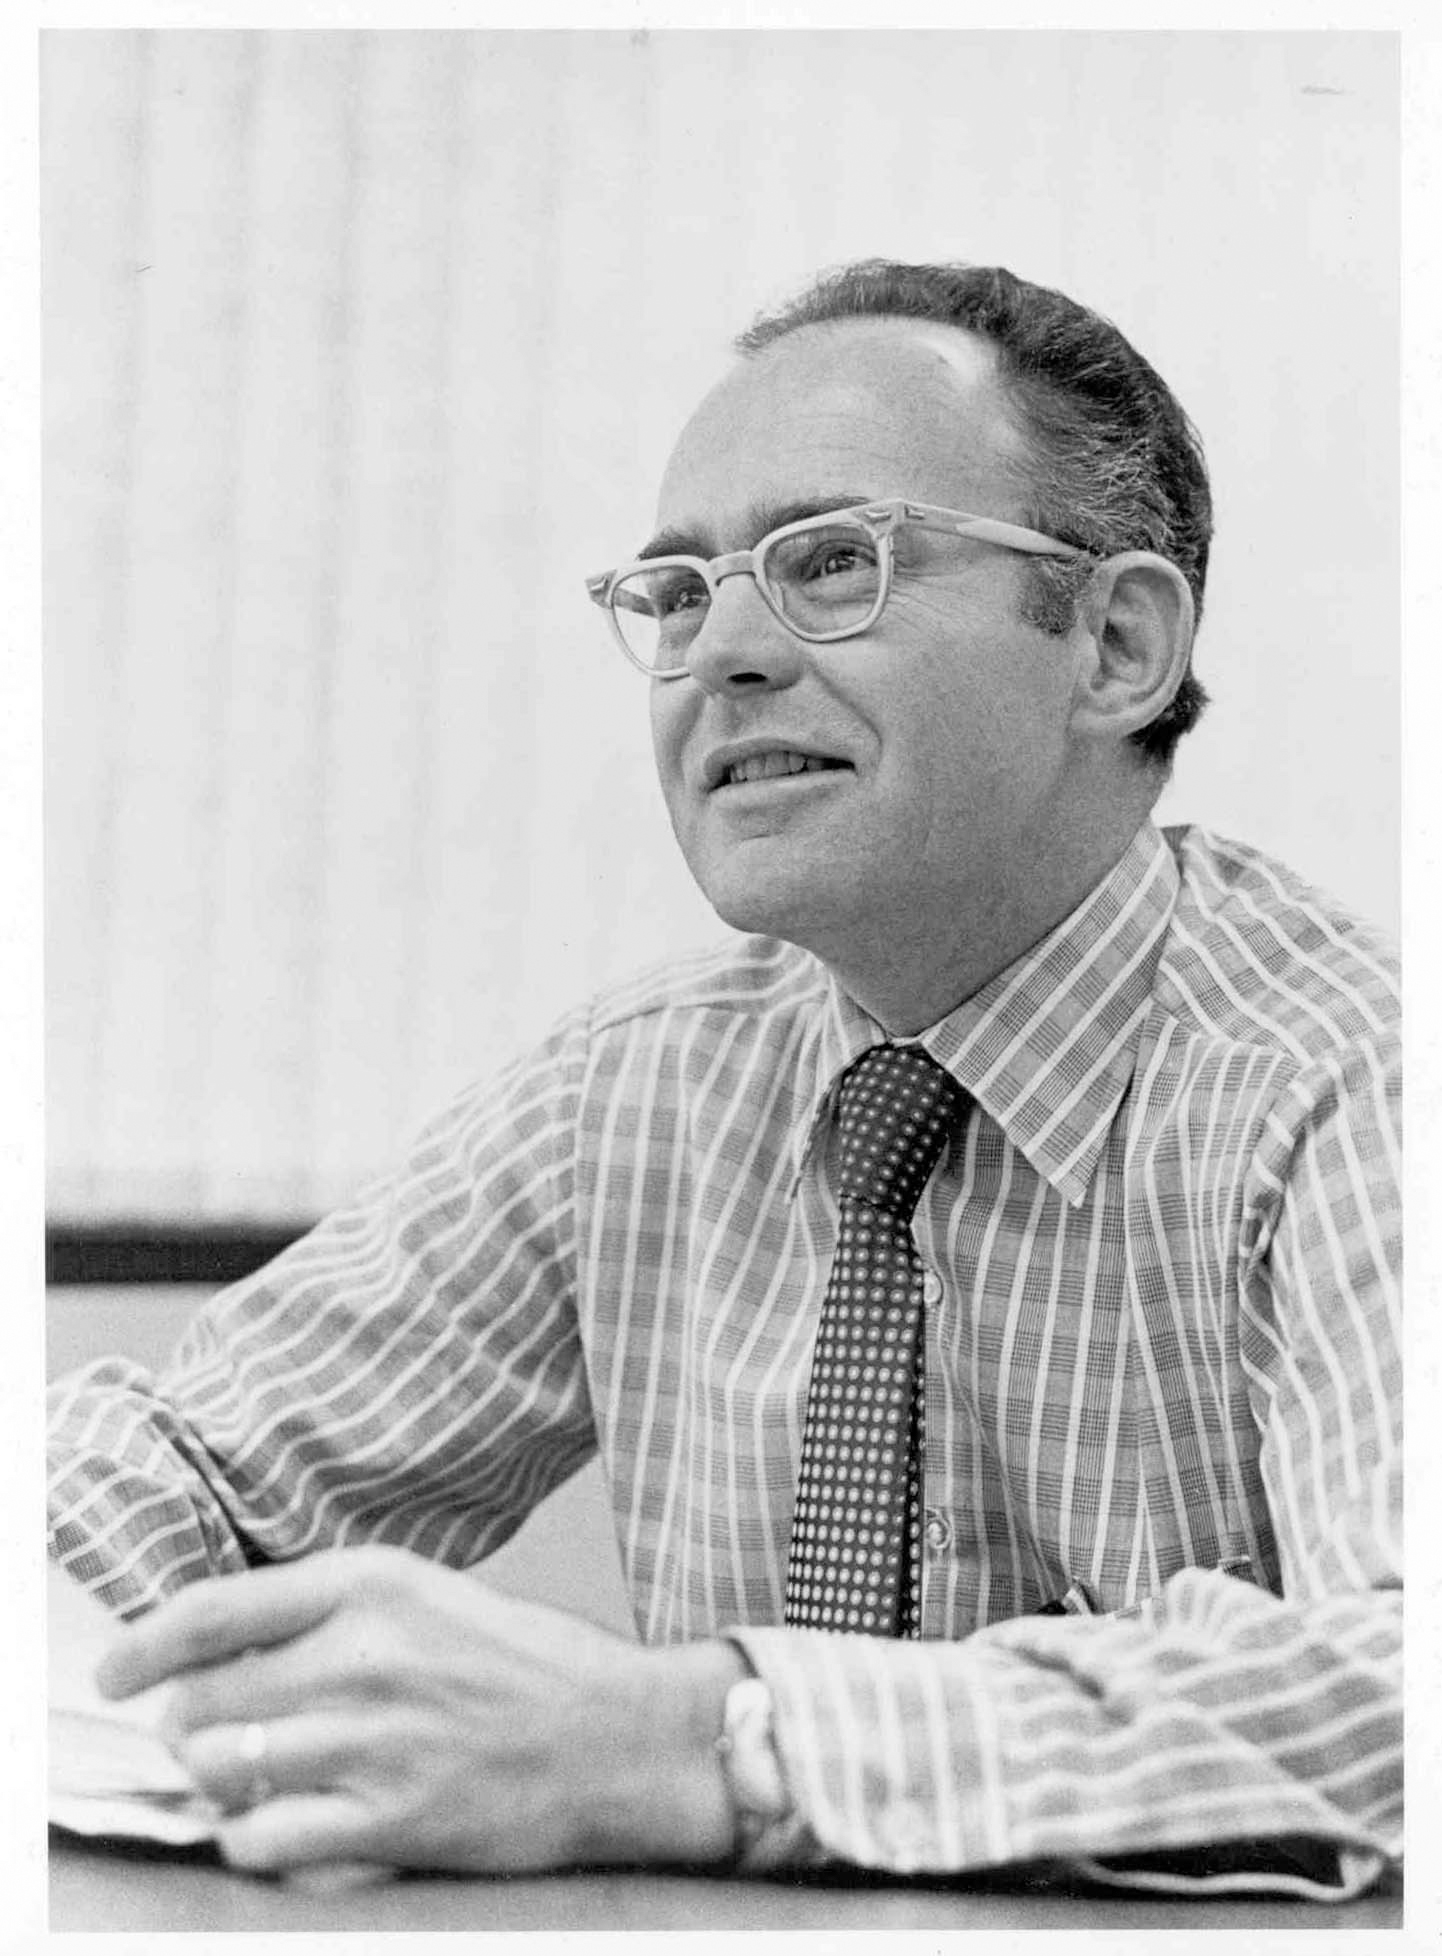
\includegraphics[height=1.5in,clip]{GordonMoore1975}
  \end{column}
\end{columns}
\end{frame}

%%%%%%%%%%%%%%%%%%%%%%%%%%%%%%%%%%%%%%%%%%%%%%%%%%%%%%
%%%%%%%%%%%%%%%%%%%%%%%%%%%%%%%%%%%%%%%%%%%%%%%%%%%%%%
\begin{frame}{Moore's ``Law"}

\begin{figure}
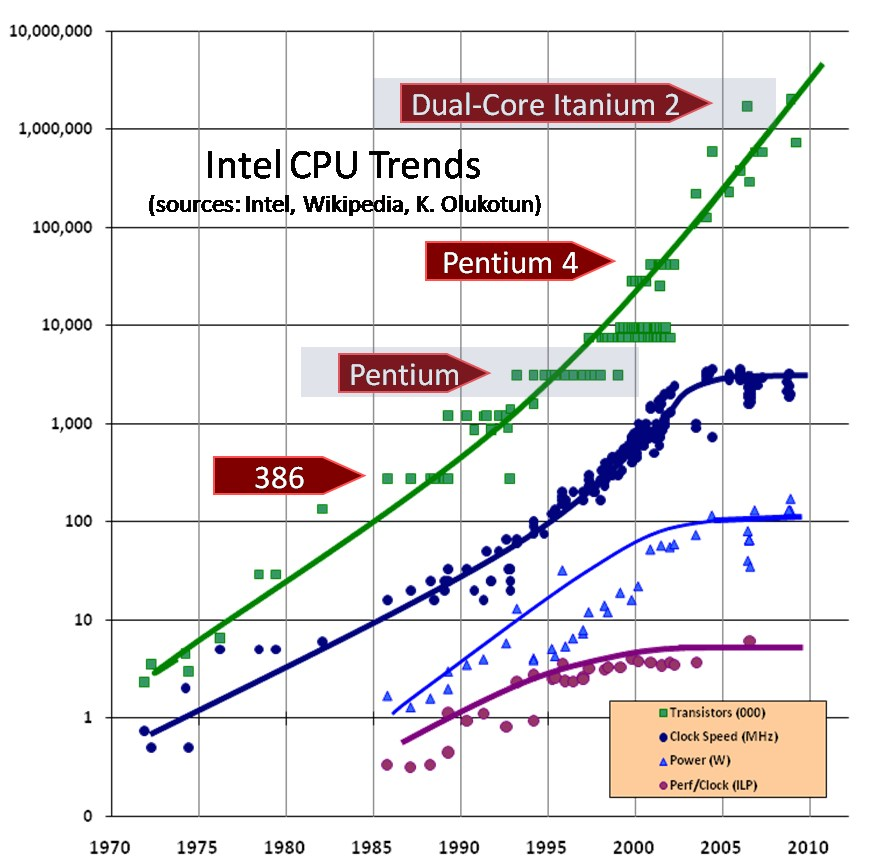
\includegraphics[height=2.75in,clip]{CPU-Scaling}
%\caption{CPU scaling showing transistor density, power consumption, and efficiency, http://www.extremetech.com/computing/116561-the-death-of-cpu-scaling-from-one-core-to-many-and-why-were-still-stuck}
\end{figure}

\end{frame}

%%%%%%%%%%%%%%%%%%%%%%%%%%%%%%%%%%%%%%%%%%%%%%%%%%%%%%
%%%%%%%%%%%%%%%%%%%%%%%%%%%%%%%%%%%%%%%%%%%%%%%%%%%%%%
\section{\scshape Parallelism}
\subsection{Parallelism}
\begin{frame}{What is Parallel Architecture?}
A \textcolor{dgreen}{parallel computer} is a collection of processing elements that cooperate to solve large problems
quickly

\begin{itemize}
\item Resource allocation
  \begin{itemize}
  \item How much \textcolor{dgreen}{memory}?
  \item How \textcolor{dgreen}{many} elements?
  \item How \textcolor{dgreen}{powerful} are the elements?
  \end{itemize}
\item Data access, Communication, and Synchronization
  \begin{itemize}
  \item How do the elements cooperate and \textcolor{dgreen}{communicate}?
  \item How are \textcolor{dgreen}{data transmitted} between processors?
  \item What are the \textcolor{dgreen}{abstractions} and primitives for cooperation?
  \end{itemize}
\item Performance and Scalability
  \begin{itemize}
  \item How does it all translate into \textcolor{dgreen}{performance}?
  \item How does it \textcolor{dgreen}{scale}?
  \end{itemize}
\end{itemize}

\end{frame}

%%%%%%%%%%%%%%%%%%%%%%%%%%%%%%%%%%%%%%%%%%%%%%%%%%%%%%
%%%%%%%%%%%%%%%%%%%%%%%%%%%%%%%%%%%%%%%%%%%%%%%%%%%%%%
\begin{frame}{Forms of Parallelism}
\begin{itemize}
\item \textbf{Bit level}: increases in word size reduced the \# of instructions the processor needs
\item \textbf{Instruction level}: hardware and/or software perform operations simultaneously when possible
\item \textbf{Memory system}: overlap of memory operations with computation
\item \textbf{Operating system}: multiple jobs run in parallel on commodity symmetric multiprocessors (SMPs) 
\end{itemize}
There are limitations to all of these

\vspace*{1 em}
To achieve high performance, the programmer needs to identify, schedule, and coordinate parallel tasks and data

\end{frame}

%%%%%%%%%%%%%%%%%%%%%%%%%%%%%%%%%%%%%%%%%%%%%%%%%%%%%%
%%%%%%%%%%%%%%%%%%%%%%%%%%%%%%%%%%%%%%%%%%%%%%%%%%%%%%
\begin{frame}{Performance}

\begin{columns}
  \begin{column}{0.65\textwidth}
\begin{itemize}
\item \textbf{Strong Scaling}: increase element count with problems size fixed (solve a problem faster)\\
\vspace*{0.5 em}
$Speedup = \frac{\text{Time with P cores}}{\text{Time with 1 core}}$
\item \textbf{Weak Scaling}: increase element count and problem size to keep problem size per element fixed (solve bigger problems)\\
\vspace*{0.5 em}
$Speedup = \frac{\text{Time with 1 core}}{\text{Time with P cores}}$
\end{itemize}
  \end{column}
  \begin{column}{0.35\textwidth}
    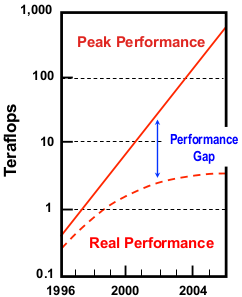
\includegraphics[height=2in,clip]{PerformanceGap}
  \end{column}
\end{columns}

\end{frame}

%%%%%%%%%%%%%%%%%%%%%%%%%%%%%%%%%%%%%%%%%%%%%%%%%%%%%%
%%%%%%%%%%%%%%%%%%%%%%%%%%%%%%%%%%%%%%%%%%%%%%%%%%%%%%
\begin{frame}{Types of Memory}

%\begin{itemize}
%\item \textbf{Shared Memory}: single memory space used by all processors; processors do not have to know where data resides
%\item \textbf{Distributed Memory}: each processor has its own private memory; tasks can only operate on local data; communication with a remote processor to get remote data
%\item \textbf{Distributed Shared Memory}: each node of a cluster has access to a large shared memory in addition to each node's limited non-shared private memory.
%\end{itemize}
\begin{center}
Shared \hspace*{2 em} Distributed \hspace*{2 em} Distributed Shared
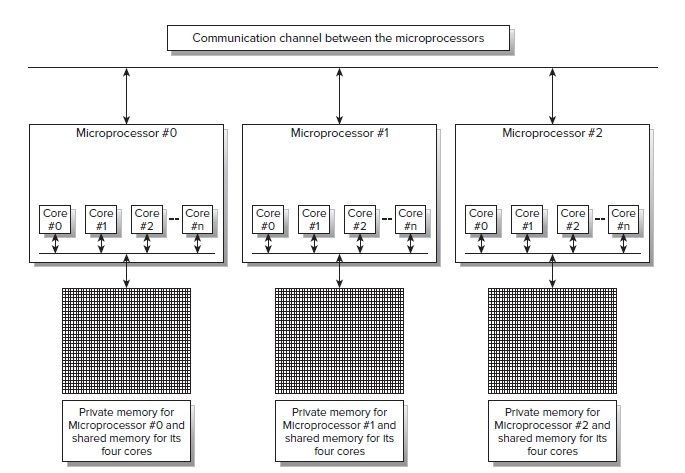
\includegraphics[height=2.5in,clip]{MemorySystems}
\end{center}

\end{frame}

%%%%%%%%%%%%%%%%%%%%%%%%%%%%%%%%%%%%%%%%%%%%%%%%%%%%%%
%%%%%%%%%%%%%%%%%%%%%%%%%%%%%%%%%%%%%%%%%%%%%%%%%%%%%%
\begin{frame}{GPUs}
\begin{itemize}
\item Graphics Processing Unit (\textbf{GPU}): highly parallel, good for processing large blocks of data
\item General Purpose GPU (\textbf{GPGPU}): Using a GPU to do CPU work - computational science instead of graphics
\end{itemize}

\begin{center}
NVIDIA GPU \\ \vspace*{1 em}
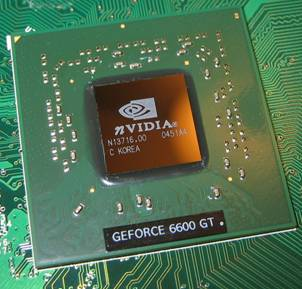
\includegraphics[height=1.5in,clip]{GPU}
\end{center}
\end{frame}

%%%%%%%%%%%%%%%%%%%%%%%%%%%%%%%%%%%%%%%%%%%%%%%%%%%%%%
%%%%%%%%%%%%%%%%%%%%%%%%%%%%%%%%%%%%%%%%%%%%%%%%%%%%%%
\begin{frame}{MICs}
\begin{itemize}
\item  Many Integrated Core (\textbf{MIC}): combines many Intel CPU cores onto a single chip
\item \textbf{Heterogeneous} architecture: GPUs + CPUs or MICs + CPUs, etc.
\end{itemize}

\begin{center}
Intel Xeon Phi Board\\ \vspace*{1 em}
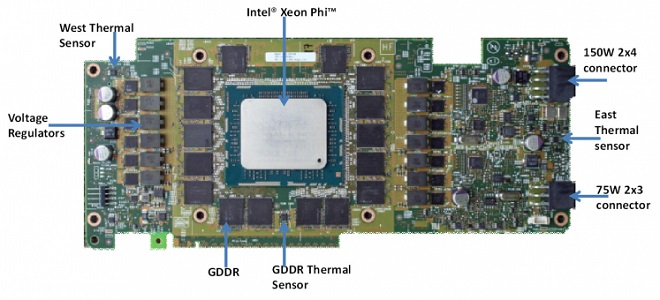
\includegraphics[height=1.75in,clip]{Intel-Xeon-Phi-Board}
\end{center}
\end{frame}

%%%%%%%%%%%%%%%%%%%%%%%%%%%%%%%%%%%%%%%%%%%%%%%%%%%%%%
%%%%%%%%%%%%%%%%%%%%%%%%%%%%%%%%%%%%%%%%%%%%%%%%%%%%%%
\section{\scshape Supercomputing}
\subsection{Supercomputing}
\begin{frame}{Scientific Computing Demand}

\begin{center}
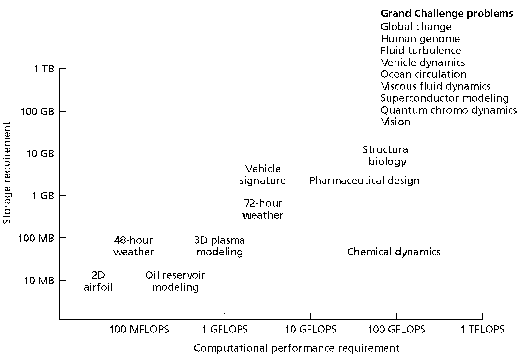
\includegraphics[height=2.75in,clip]{MemoryNeeds}
\end{center}

\end{frame}

%%%%%%%%%%%%%%%%%%%%%%%%%%%%%%%%%%%%%%%%%%%%%%%%%%%%%%
%%%%%%%%%%%%%%%%%%%%%%%%%%%%%%%%%%%%%%%%%%%%%%%%%%%%%%
\begin{frame}{\href{http://www.top500.org/list/2014/11/}{Top 500 Computers, Nov 2014}}

\begin{center}
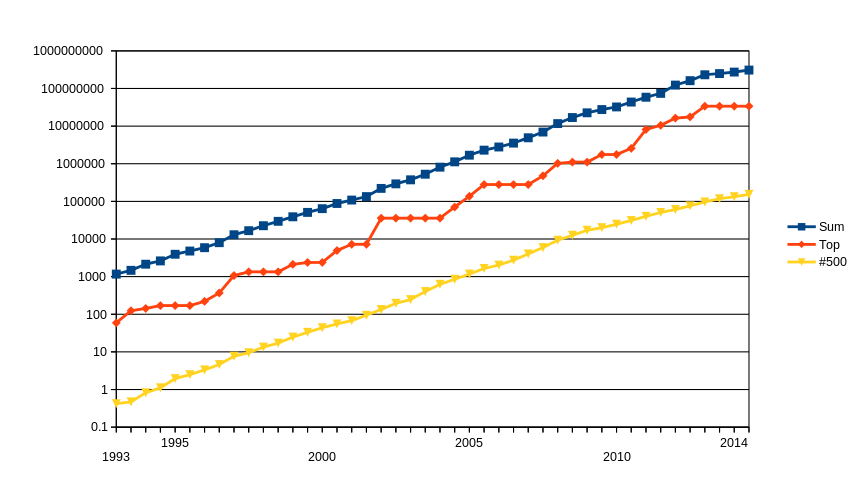
\includegraphics[height=2.5in]{Supercomputers-history}
Log y axis in GFLOPS, x axis in years
\end{center}

\end{frame}

%%%%%%%%%%%%%%%%%%%%%%%%%%%%%%%%%%%%%%%%%%%%%%%%%%%%%%
%%%%%%%%%%%%%%%%%%%%%%%%%%%%%%%%%%%%%%%%%%%%%%%%%%%%%%
\begin{frame}{\href{http://en.wikipedia.org/wiki/TOP500}{Top 10 Computers, Nov 2014}}

\begin{center}
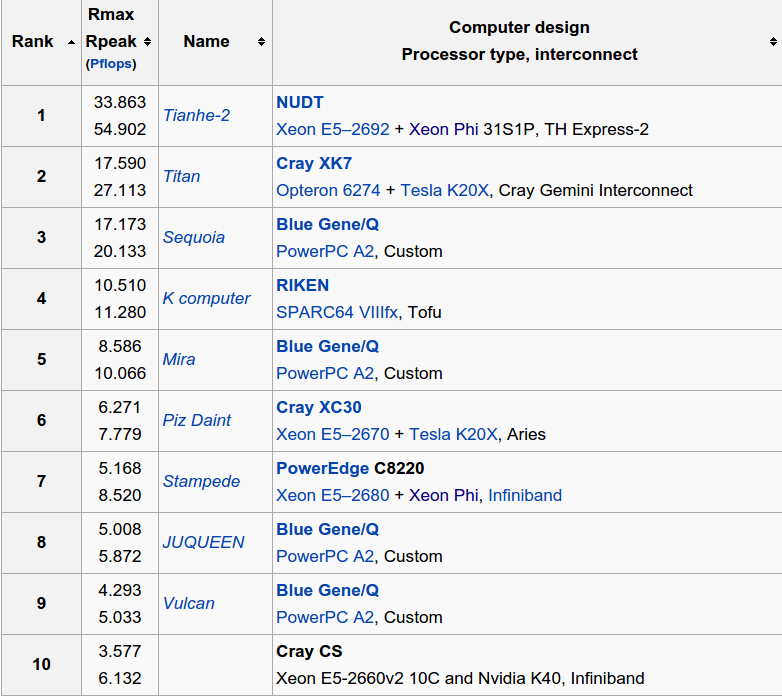
\includegraphics[height=3in]{2014-top-10}
\end{center}

%Look at the \href{http://www.top500.org/statistics/efficiency-power-cores/}{Power and Efficiency} trends.

\end{frame}

%%%%%%%%%%%%%%%%%%%%%%%%%%%%%%%%%%%%%%%%%%%%%%%%%%%%%%
%%%%%%%%%%%%%%%%%%%%%%%%%%%%%%%%%%%%%%%%%%%%%%%%%%%%%%
\begin{frame}{Power Consumption, Nov 2013}

\begin{center}
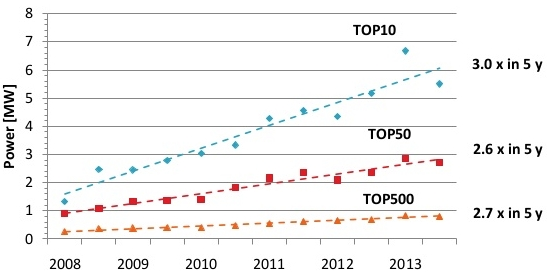
\includegraphics[height=2.25in]{Top500-power}
\end{center}

\end{frame}

%%%%%%%%%%%%%%%%%%%%%%%%%%%%%%%%%%%%%%%%%%%%%%%%%%%%%%
%%%%%%%%%%%%%%%%%%%%%%%%%%%%%%%%%%%%%%%%%%%%%%%%%%%%%%
\begin{frame}{Power Efficiency, Nov 2013}

\begin{center}
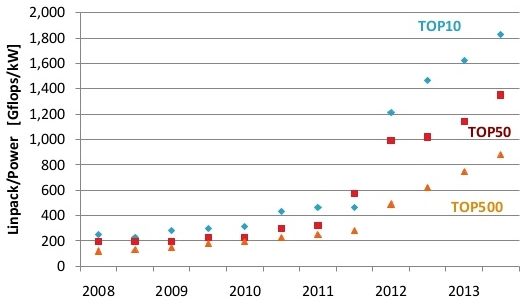
\includegraphics[height=2.25in]{Top500-efficiency}
\end{center}

\end{frame}


%%%%%%%%%%%%%%%%%%%%%%%%%%%%%%%%%%%%%%%%%%%%%%%%%%%%%%
%%%%%%%%%%%%%%%%%%%%%%%%%%%%%%%%%%%%%%%%%%%%%%%%%%%%%%
\begin{frame}{Where are we going?}
\begin{center}
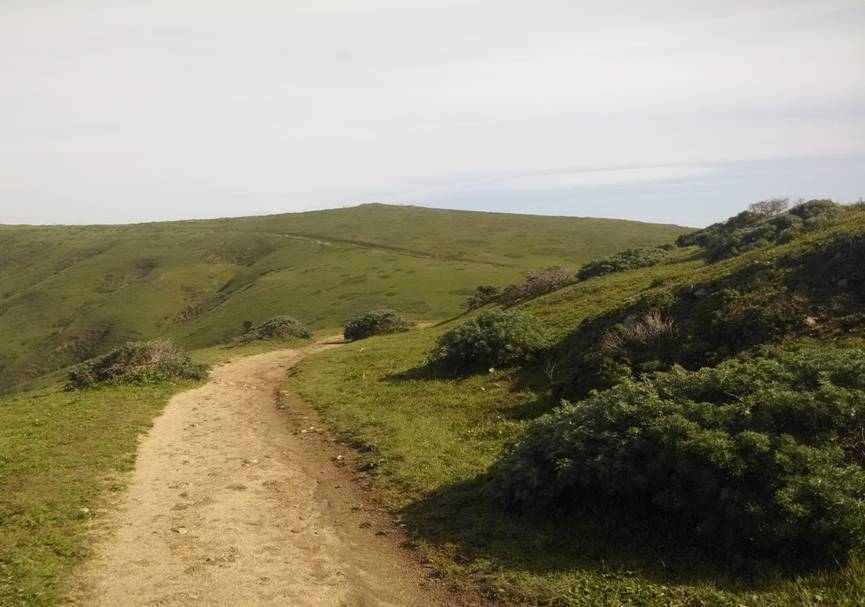
\includegraphics[height=2.25in]{road}
\end{center}
\end{frame}

%%%%%%%%%%%%%%%%%%%%%%%%%%%%%%%%%%%%%%%%%%%%%%%%%%%%%%
%%%%%%%%%%%%%%%%%%%%%%%%%%%%%%%%%%%%%%%%%%%%%%%%%%%%%%
\section*{}
\begin{frame}{Recap}
\begin{itemize}
\item Humans have been working to use machines for computation for a very long time
\item The 20th century saw the development of the computers we know today $\rightarrow$ development of computational science as a field
\item A revolution in supercomputing began at the end of the 20th century $\rightarrow$ \alert{computational science is a major contributor to knowledge}
\item We are reaching the limits of ``traditional" architecture growth
\item What we can compute and how is tightly tied to computer architecture development
\end{itemize}
\end{frame}

\end{document}